
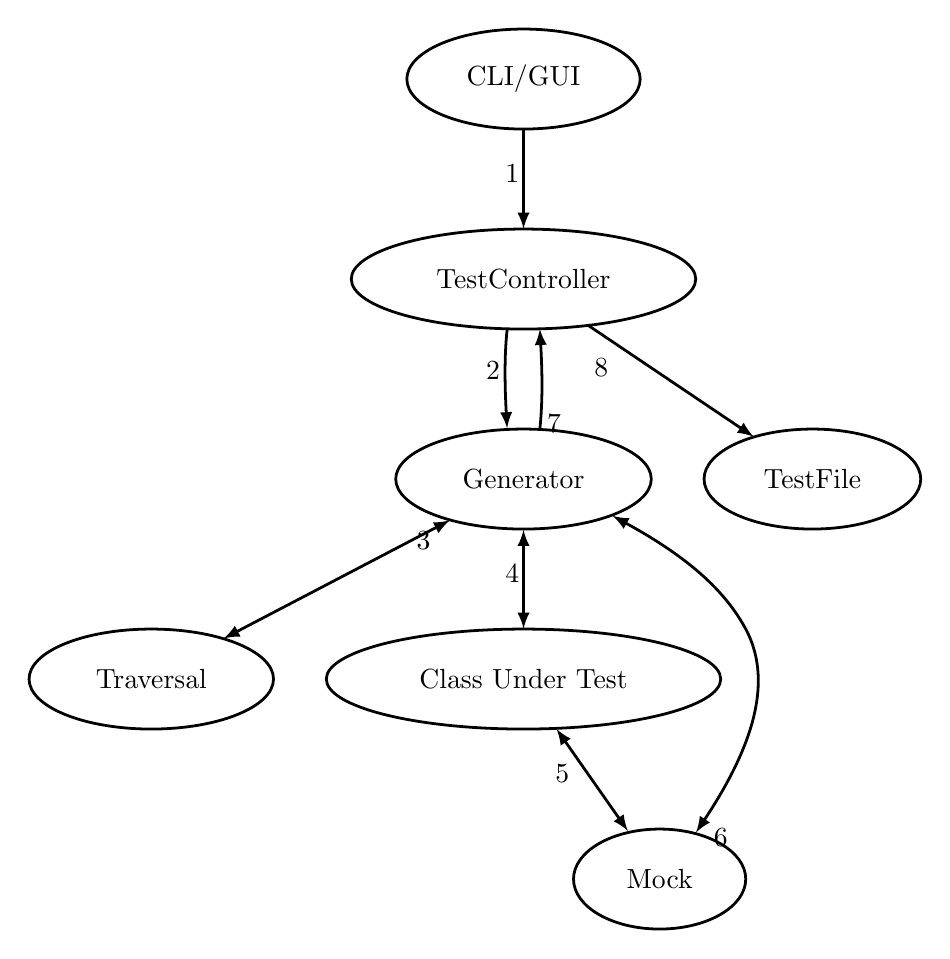
\begin{tikzpicture}[>=latex,line join=bevel,]
  \pgfsetlinewidth{1bp}
%%
\pgfsetcolor{black}
  % Edge: Generator -> TestController
  \draw [->] (183.91bp,180.28bp) .. controls (184.71bp,188.03bp) and (184.94bp,197.36bp)  .. (183.88bp,216.05bp);
  \definecolor{strokecol}{rgb}{0.0,0.0,0.0};
  \pgfsetstrokecolor{strokecol}
  \draw (189bp,182bp) node {7};
  % Edge: TestController -> TestFile
  \draw [->] (201.34bp,217.29bp) .. controls (216.4bp,207.16bp) and (236.12bp,193.88bp)  .. (260.86bp,177.23bp);
  \draw (206bp,202bp) node {8};
  % Edge: Class Under Test -> Mock
  \draw [<->] (189.86bp,72.055bp) .. controls (200.24bp,57.222bp) and (205.14bp,50.222bp)  .. (215.59bp,35.307bp);
  \draw (192bp,56bp) node {5};
  % Edge: CLI/GUI -> TestController
  \draw [->] (178bp,287.7bp) .. controls (178bp,279.98bp) and (178bp,270.71bp)  .. (178bp,252.1bp);
  \draw (174bp,272bp) node {1};
  % Edge: TestController -> Generator
  \draw [->] (172.12bp,216.05bp) .. controls (171.3bp,208.35bp) and (171.06bp,199.03bp)  .. (172.09bp,180.28bp);
  \draw (167bp,201bp) node {2};
  % Edge: Generator -> Class Under Test
  \draw [<->] (178bp,143.7bp) .. controls (178bp,128.69bp) and (178bp,123.49bp)  .. (178bp,108.1bp);
  \draw (174bp,128bp) node {4};
  % Edge: Generator -> Traversal
  \draw [<->] (151.53bp,147.17bp) .. controls (122.82bp,132.17bp) and (98.445bp,119.44bp)  .. (69.963bp,104.56bp);
  \draw (142bp,140bp) node {3};
  % Edge: Mock -> Generator
  \draw [<->] (240.08bp,34.735bp) .. controls (257.89bp,61.544bp) and (269.18bp,87.189bp)  .. (258bp,108bp) .. controls (249.58bp,123.68bp) and (234.26bp,135.5bp)  .. (210.02bp,148.79bp);
  \draw (249bp,33bp) node {6};
  % Node: CLI/GUI
\begin{scope}
  \definecolor{strokecol}{rgb}{0.0,0.0,0.0};
  \pgfsetstrokecolor{strokecol}
  \draw (178bp,306bp) ellipse (42bp and 18bp);
  \draw (178bp,306bp) node {CLI/GUI};
\end{scope}
  % Node: Generator
\begin{scope}
  \definecolor{strokecol}{rgb}{0.0,0.0,0.0};
  \pgfsetstrokecolor{strokecol}
  \draw (178bp,162bp) ellipse (46bp and 18bp);
  \draw (178bp,162bp) node {Generator};
\end{scope}
  % Node: Class Under Test
\begin{scope}
  \definecolor{strokecol}{rgb}{0.0,0.0,0.0};
  \pgfsetstrokecolor{strokecol}
  \draw (178bp,90bp) ellipse (71bp and 18bp);
  \draw (178bp,90bp) node {Class Under Test};
\end{scope}
  % Node: Traversal
\begin{scope}
  \definecolor{strokecol}{rgb}{0.0,0.0,0.0};
  \pgfsetstrokecolor{strokecol}
  \draw (44bp,90bp) ellipse (44bp and 18bp);
  \draw (44bp,90bp) node {Traversal};
\end{scope}
  % Node: TestController
\begin{scope}
  \definecolor{strokecol}{rgb}{0.0,0.0,0.0};
  \pgfsetstrokecolor{strokecol}
  \draw (178bp,234bp) ellipse (62bp and 18bp);
  \draw (178bp,234bp) node {TestController};
\end{scope}
  % Node: TestFile
\begin{scope}
  \definecolor{strokecol}{rgb}{0.0,0.0,0.0};
  \pgfsetstrokecolor{strokecol}
  \draw (282bp,162bp) ellipse (39bp and 18bp);
  \draw (282bp,162bp) node {TestFile};
\end{scope}
  % Node: Mock
\begin{scope}
  \definecolor{strokecol}{rgb}{0.0,0.0,0.0};
  \pgfsetstrokecolor{strokecol}
  \draw (227bp,18bp) ellipse (31bp and 18bp);
  \draw (227bp,18bp) node {Mock};
\end{scope}
%
\end{tikzpicture}

